% Options for packages loaded elsewhere
\PassOptionsToPackage{unicode}{hyperref}
\PassOptionsToPackage{hyphens}{url}
%
\documentclass[
  12pt,
]{article}
\usepackage{amsmath,amssymb}
\usepackage{iftex}
\ifPDFTeX
  \usepackage[T1]{fontenc}
  \usepackage[utf8]{inputenc}
  \usepackage{textcomp} % provide euro and other symbols
\else % if luatex or xetex
  \usepackage{unicode-math} % this also loads fontspec
  \defaultfontfeatures{Scale=MatchLowercase}
  \defaultfontfeatures[\rmfamily]{Ligatures=TeX,Scale=1}
\fi
\usepackage{lmodern}
\ifPDFTeX\else
  % xetex/luatex font selection
\fi
% Use upquote if available, for straight quotes in verbatim environments
\IfFileExists{upquote.sty}{\usepackage{upquote}}{}
\IfFileExists{microtype.sty}{% use microtype if available
  \usepackage[]{microtype}
  \UseMicrotypeSet[protrusion]{basicmath} % disable protrusion for tt fonts
}{}
\makeatletter
\@ifundefined{KOMAClassName}{% if non-KOMA class
  \IfFileExists{parskip.sty}{%
    \usepackage{parskip}
  }{% else
    \setlength{\parindent}{0pt}
    \setlength{\parskip}{6pt plus 2pt minus 1pt}}
}{% if KOMA class
  \KOMAoptions{parskip=half}}
\makeatother
\usepackage{xcolor}
\usepackage[margin=1in]{geometry}
\usepackage{listings}
\newcommand{\passthrough}[1]{#1}
\lstset{defaultdialect=[5.3]Lua}
\lstset{defaultdialect=[x86masm]Assembler}
\usepackage{graphicx}
\makeatletter
\def\maxwidth{\ifdim\Gin@nat@width>\linewidth\linewidth\else\Gin@nat@width\fi}
\def\maxheight{\ifdim\Gin@nat@height>\textheight\textheight\else\Gin@nat@height\fi}
\makeatother
% Scale images if necessary, so that they will not overflow the page
% margins by default, and it is still possible to overwrite the defaults
% using explicit options in \includegraphics[width, height, ...]{}
\setkeys{Gin}{width=\maxwidth,height=\maxheight,keepaspectratio}
% Set default figure placement to htbp
\makeatletter
\def\fps@figure{htbp}
\makeatother
\setlength{\emergencystretch}{3em} % prevent overfull lines
\providecommand{\tightlist}{%
  \setlength{\itemsep}{0pt}\setlength{\parskip}{0pt}}
\setcounter{secnumdepth}{-\maxdimen} % remove section numbering
% definitions for citeproc citations
\NewDocumentCommand\citeproctext{}{}
\NewDocumentCommand\citeproc{mm}{%
  \begingroup\def\citeproctext{#2}\cite{#1}\endgroup}
\makeatletter
 % allow citations to break across lines
 \let\@cite@ofmt\@firstofone
 % avoid brackets around text for \cite:
 \def\@biblabel#1{}
 \def\@cite#1#2{{#1\if@tempswa , #2\fi}}
\makeatother
\newlength{\cslhangindent}
\setlength{\cslhangindent}{1.5em}
\newlength{\csllabelwidth}
\setlength{\csllabelwidth}{3em}
\newenvironment{CSLReferences}[2] % #1 hanging-indent, #2 entry-spacing
 {\begin{list}{}{%
  \setlength{\itemindent}{0pt}
  \setlength{\leftmargin}{0pt}
  \setlength{\parsep}{0pt}
  % turn on hanging indent if param 1 is 1
  \ifodd #1
   \setlength{\leftmargin}{\cslhangindent}
   \setlength{\itemindent}{-1\cslhangindent}
  \fi
  % set entry spacing
  \setlength{\itemsep}{#2\baselineskip}}}
 {\end{list}}
\usepackage{calc}
\newcommand{\CSLBlock}[1]{\hfill\break\parbox[t]{\linewidth}{\strut\ignorespaces#1\strut}}
\newcommand{\CSLLeftMargin}[1]{\parbox[t]{\csllabelwidth}{\strut#1\strut}}
\newcommand{\CSLRightInline}[1]{\parbox[t]{\linewidth - \csllabelwidth}{\strut#1\strut}}
\newcommand{\CSLIndent}[1]{\hspace{\cslhangindent}#1}
% !TEX TS-program = xelatex
% !TEX encoding = UTF-8 Unicode

% Language, font, and typography management
\usepackage{babel, fontspec, lmodern, unicode-math, microtype}
\usepackage{amsmath, amssymb, gensymb, xcolor}

% Page layout and formatting
\geometry{a4paper, left=1in, right=1in, top=1in, bottom=1in, headheight=0.5in, footskip=0.5in}  % Consistent margin setting
\usepackage{setspace}  % For controlling line spacing
\setlength{\parskip}{8pt plus 2pt minus 1pt}  % More comfortable paragraph spacing
\setstretch{1.5}  % Adjust line spacing to 1.5 for better readability

% Section title formatting
\usepackage{titlesec}  % Title formatting
\titleformat{\section}[block]{\Large\bfseries\centering}{\thesection}{1em}{}  % Section header formatting
\titleformat{\subsection}[runin]{\large\bfseries}{\thesubsection}{1em}{}  % Subsection formatting with inline style
\titleformat{\subsubsection}[runin]{\normalsize\bfseries}{\thesubsubsection}{1em}{}  % Subsubsection inline formatting

% Additional improvements for section and subsection spacing
\titlespacing*{\section}{0pt}{12pt plus 4pt minus 2pt}{8pt plus 2pt minus 2pt}  % Adjust space before and after sections
\titlespacing*{\subsection}{0pt}{8pt plus 2pt minus 1pt}{6pt plus 1pt minus 1pt}  % Adjust space before and after subsections
\titlespacing*{\subsubsection}{0pt}{6pt plus 1pt minus 1pt}{4pt plus 1pt minus 1pt}  % Adjust space before and after subsubsections

% Additional document settings for clarity
\setlength{\parindent}{0pt}  % Remove paragraph indentation (for better readability with increased line spacing)
\setlength{\emergencystretch}{3em}  % Prevent overfull lines by stretching a bit

% Header and footer setup
\usepackage{fancyhdr}
\pagestyle{fancy}
% Left/Right header (empty)
\fancyhead[L,R]{}  
% Left/Right header (empty)
\fancyfoot[L,R]{}  
% center of header
\fancyhead[C]{Rmarkdown Template File}
% center of footer
\fancyfoot[C]{\thepage}

\definecolor{urbnblue}{HTML}{1696D2}    % Defines the blue color


% Listings for code formatting (R code)
\usepackage{listings}
\usepackage{xcolor}  % For color customization
\lstdefinestyle{RStyle}{
  language=R,                         % Set the language to R
  backgroundcolor=\color{gray!10},  % Set background color
  basicstyle=\fontsize{10}{11}\selectfont\ttfamily,  % Custom font size between tiny and small
  backgroundcolor=\color{white},      % Set background color
  showspaces=false,                   % Do not display spaces with underscores
  showstringspaces=false,             % Do not underline spaces in strings
  showtabs=false,                     % Do not display tabs with arrows
  tabsize=2,                          % Set tab size to 2 spaces
  breaklines=true,                    % Enable line breaking
  breakautoindent=true,             % Enable auto-indentation after line breaks
  columns=fullflexible,             % Use full flexible column width
  xleftmargin=15pt, xrightmargin=15pt,  % Adjust code block margins
  commentstyle=\color{urbnblue},          % Style for comments
  keywordstyle=\color{black},          % Style for keywords
  stringstyle=\color{gray}           % Style for strings
}
\lstset{style=RStyle}

% Fancy verbatim (improve code formatting)
\usepackage{fancyvrb}
\usepackage{fvextra}
\DefineVerbatimEnvironment{Highlighting}{Verbatim}{
    breaklines=true,
    breakanywhere=true,
    commandchars=\\\{\},
    fontsize=\small
}

% Hyperlink and references setup
\usepackage{hyperref}  % Hyperlinks and references
\hypersetup{
  colorlinks=true,
  linkcolor=urbnblue,
  citecolor=urbnblue,
  urlcolor=urbnblue,
  pdfborder={0 0 0}
}

% Tables and long tables
\usepackage{longtable,booktabs}

% Graphics and figures
\usepackage{graphicx}
\makeatletter
\def\maxwidth{\ifdim\Gin@nat@width>\linewidth\linewidth\else\Gin@nat@width\fi}
\def\maxheight{\ifdim\Gin@nat@height>\textheight\textheight\else\Gin@nat@height\fi}
\makeatother
\setkeys{Gin}{width=\maxwidth,height=\maxheight,keepaspectratio}

% The rest of the document content will go here. 
\ifLuaTeX
  \usepackage{selnolig}  % disable illegal ligatures
\fi
\usepackage{bookmark}
\IfFileExists{xurl.sty}{\usepackage{xurl}}{} % add URL line breaks if available
\urlstyle{same}
\hypersetup{
  pdftitle={RMarkdown Template File},
  pdfauthor={Robert J. Dellinger},
  hidelinks,
  pdfcreator={LaTeX via pandoc}}

\title{RMarkdown Template File}
\author{Robert J. Dellinger}
\date{April 06, 2025}

\begin{document}
\maketitle

{
\setcounter{tocdepth}{3}
\tableofcontents
}
\newpage

\section{Introduction}\label{introduction}

This document outlines the methodology for data cleaning, exploration,
and visualization. It is structured to ensure transparency and
reproducibility of all analyses.

\subsection{Methodology}\label{methodology}

Briefly describe the methods used in the project, including data
sources, cleaning steps, and techniques applied to handle missing or
inconsistent data.

\subsubsection{Math Equations with
LaTeX}\label{math-equations-with-latex}

Here is an inline equation: \(E = mc^2\).

And here is a displayed equation:

\begin{equation}
f(x) = \int_{-\infty}^{\infty} e^{-x^2} \, dx
\end{equation}

Both inline and block math can be rendered seamlessly with LaTeX.

You can also create multiline equations with alignment:

\begin{equation}
\begin{aligned}
a &= b + c \\
d &= e + f
\end{aligned}
\end{equation}

\subsection{Setup Packages}\label{setup-packages}

The first step in any data analysis is to load the data, options, and
packages. This section installs and loads the necessary packages, sets
up the output paths, and defines chunk options for the RMarkdown
document.

\subsection{Loading Data}\label{loading-data}

The following code loads the data from various sources, including CSV
files, Excel files, and shapefiles. The \passthrough{\lstinline!here!}
package is used to create file paths that are relative to the project
directory, ensuring that the code is portable and reproducible.

\begin{lstlisting}[language=R]
# Example of loading data from a CSV file
# raw_data <- read_csv(here("Data", "Raw", "data_file.csv"))
# raw_data <- read_excel(here("Data", "Raw", "data_file.xlsx"))
# raw_data <- read_sf(here("Data", "Raw", "data_file.shp"))
\end{lstlisting}

\subsection{Cleaning Data}\label{cleaning-data}

The data cleaning process involves several steps to ensure the data is
in a suitable format for analysis. This includes handling missing
values, correcting data types, and removing duplicates.

\begin{lstlisting}[language=R]
# cleaning the data using dplyr and tidyr
# cleaned_data <- raw_data %>%
#   clean_names() %>%
#   mutate(column_name = as_factor(column_name)) %>% 
#   mutate(date_column = as.Date(date_column, format = "%Y-%m-%d")) %>% 
#   mutate(numeric_column = as.numeric(numeric_column)) %>% 
#   mutate(accross(everything(), ~str_squish(.))) %>% =
#   drop_na()
\end{lstlisting}

\subsection{Data Exploration}\label{data-exploration}

Data exploration is a crucial step in understanding the dataset and
identifying patterns or anomalies. This section includes summary
statistics, visualizations, and any other relevant analyses to gain
insights into the data.

\begin{lstlisting}[language=R]
# Explore the cleaned data using basic summaries:
# glimpse(cleaned_data)
# summary(cleaned_data)
# str(cleaned_data)
\end{lstlisting}

\subsection{Data Visualization}\label{data-visualization}

Data visualization is an essential part of data analysis, allowing for
the communication of findings in a clear and effective manner. This
section includes various plots and charts to illustrate key insights
from the data.

\begin{lstlisting}[language=R]
# Example of creating a summary table 
# summary_table <- cleaned_data %>%
#   group_by(group_var) %>%
#   summarise(mean_value = mean(value_var, na.rm = TRUE)) %>%
#   ungroup() %>%
#   kable() %>%
#   kable_styling(full_width = F, position = "left") 

# save_kable(summary_table, file = here(output_path_tables, "summary_table.html"),
#   bootstrap_options = c("striped", "hover", "condensed"),
#   full_width = F, position = "left")
\end{lstlisting}

\begin{lstlisting}[language=R]
# Example of visualization plot
data("diamonds")

# First Plot (p1) - Scatter plot with smoothing line
p1 <- ggplot(
  subset(diamonds, carat >= 2.2),
  aes(x = table, y = price, colour = cut)
) +
  geom_point(alpha = 0.7) +  
  geom_smooth(method = "loess", alpha = 0.05,
  linewidth = 1, span = 1, formula = y ~ x) +  
  theme_bw() +  # White background theme
  theme(
    plot.title = element_text(hjust = 0.5),  # Center the title
    legend.position = "top",  # Position the legend at the top
    text = element_text(size = 10),  # Set text size
    legend.key.size = unit(0.5, "cm")  # Legend key size
  )

# Second Plot (p2) - Histogram of depth for specific carat ranges
p2 <- ggplot(
  subset(diamonds, carat > 2.2 & depth > 55 & depth < 70),
  aes(x = depth, fill = cut)
) +
  geom_histogram(colour = "black",
  binwidth = 1, position = "dodge") +  # Dodged histogram
  theme_bw() +  # White background theme
  theme(
    plot.title = element_text(hjust = 0.5),  # Center the title
    legend.position = "top",  # Position the legend at the top
    text = element_text(size = 10),  # Set text size
    legend.key.size = unit(0.5, "cm")  # Legend key size
  )

p1_npg <- p1 + scale_color_npg()
p2_npg <- p2 + scale_fill_npg()
grid.arrange(p1_npg, p2_npg, ncol = 2)
\end{lstlisting}

\begin{figure}

{\centering 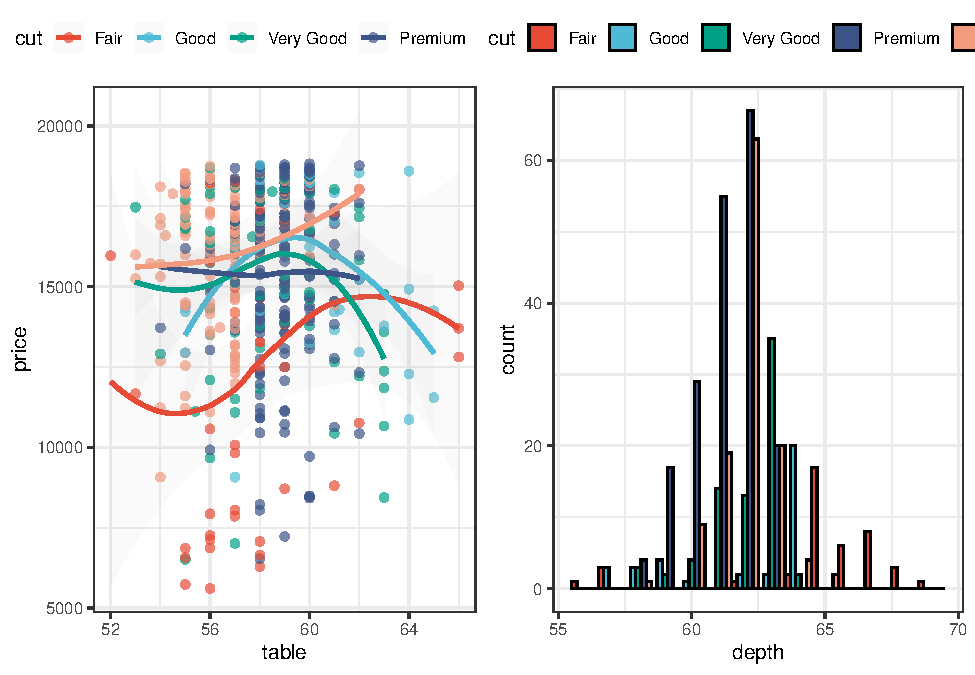
\includegraphics[width=0.8\linewidth]{/Users/robertjdellinger/Library/Mobile Documents/com~apple~CloudDocs/Documents/Applications/Github/template-repository/Output/Figures/Fig-data-visualization-plot-1} 

}

\caption{Example of a scatter plot}\label{fig:data-visualization-plot}
\end{figure}

\begin{lstlisting}[language=R]
# Example of saving a plot
# ggsave(filename = here(output_path_images, "plot_name.png"), 
# plot = last_plot(), width = 6, height = 4)
\end{lstlisting}

\clearpage
\newpage

\section{Literature Cited}\label{literature-cited}

Citing the packages and data used in the analysis is important for
reproducibility and transparency. The following code generates a
bibliography of all loaded packages. Items can be cited directly within
the documentation using the syntax \passthrough{\lstinline!@key!} where
key is the citation key in the first line of the entry, e.g., R Core
Team (2024), Wickham et al. (2024), Wickham (2023), Müller (2020). To
put citations in parentheses, use \passthrough{\lstinline![@key]!}
instead.

\phantomsection\label{refs}
\begin{CSLReferences}{1}{0}
\bibitem[\citeproctext]{ref-R-here}
Müller, K. (2020). \emph{Here: A simpler way to find your files}.
\url{https://here.r-lib.org/}

\bibitem[\citeproctext]{ref-R-base}
R Core Team. (2024). \emph{R: A language and environment for statistical
computing}. R Foundation for Statistical Computing.
\url{https://www.R-project.org/}

\bibitem[\citeproctext]{ref-R-tidyverse}
Wickham, H. (2023). \emph{Tidyverse: Easily install and load the
tidyverse}. \url{https://tidyverse.tidyverse.org}

\bibitem[\citeproctext]{ref-R-ggplot2}
Wickham, H., Chang, W., Henry, L., Pedersen, T. L., Takahashi, K.,
Wilke, C., Woo, K., Yutani, H., Dunnington, D., \& van den Brand, T.
(2024). \emph{ggplot2: Create elegant data visualisations using the
grammar of graphics}. \url{https://ggplot2.tidyverse.org}

\end{CSLReferences}

\end{document}
